\iffalse
\let\negmedspace\undefined
\let\negthickspace\undefined
\documentclass[journal,12pt,twocolumn]{IEEEtran}
\usepackage{cite}
\usepackage{amsmath,amssymb,amsfonts,amsthm}
\usepackage{algorithmic}
\usepackage{graphicx}
\usepackage{textcomp}
\usepackage{xcolor}
\usepackage{txfonts}
\usepackage{listings}
\usepackage{enumitem}
\usepackage{mathtools}
\usepackage{gensymb}
\usepackage{comment}
\usepackage[breaklinks=true]{hyperref}
\usepackage{tkz-euclide} 
\usepackage{listings}
\usepackage{gvv}                                        
\def\inputGnumericTable{}                                 
\usepackage[latin1]{inputenc}                                
\usepackage{color}                                            
\usepackage{array}                                            
\usepackage{longtable}                                       
\usepackage{calc}                                             
\usepackage{multirow}                                         
\usepackage{hhline}                                           
\usepackage{ifthen}                                           
\usepackage{lscape}
\usepackage{caption}
\newtheorem{theorem}{Theorem}[section]
\newtheorem{problem}{Problem}
\newtheorem{proposition}{Proposition}[section]
\newtheorem{lemma}{Lemma}[section]
\newtheorem{corollary}[theorem]{Corollary}
\newtheorem{example}{Example}[section]
\newtheorem{definition}[problem]{Definition}
\newcommand{\BEQA}{\begin{eqnarray}}
\newcommand{\EEQA}{\end{eqnarray}}
\newcommand{\define}{\stackrel{\triangle}{=}}
\theoremstyle{remark}
\newtheorem{rem}{Remark}
\begin{document}

\bibliographystyle{IEEEtran}
\vspace{3cm}

\title{10.5.2.14}
\author{EE23BTECH11003 - pranav}
\maketitle
\newpage

\bigskip
\renewcommand{\thefigure}{\arabic{figure}}
\renewcommand{\thetable}{\arabic{table}}

\textbf{Question}:A spring having with a spring constant 1200 N$m^{-1}$ is mounted on a horizontal
table as shown in Fig.A mass of 3 kg is attached to the free end of the
spring. The mass is then pulled sideways to a distance of 2.0 cm and released.\\
Determine (i) the frequency of oscillations, (ii) maximum acceleration of the mass,
and (iii) the maximum speed of the mass
\begin{figure}[h!]
    \centering
    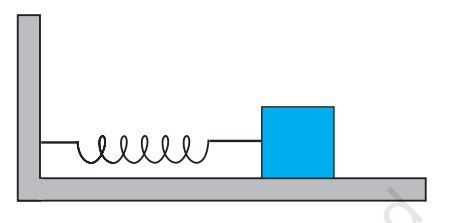
\includegraphics[width=0.5\linewidth]{ncert-physics/11/14/9/figs/figure.jpg}
    \caption{ }
    
\end{figure}\\
\solution
\fi
\begin{table}[h!]
    \centering
    \input{ncert-physics/11/14/9/tables/Table.Tex}
    \caption{Variables Used}
\end{table}
at $t=0$
\begin{align}
A&=A\sin{(\omega(0)+\phi)}\\
\implies \phi&=\frac{\pi}{2}\\
\implies x(t)&=A\cos{\omega t} 
\end{align}
\text{by appling laplace transform}
\begin{align}
X(s)&=\int_{-\infty}^{\infty} x(t)e^{-st}dt \\
\implies X(s)&=A\frac{s}{s^2+\omega^2}
\end{align}
laplace transform of $x'(t)=sX(s)-x(0)$
\begin{align}
 \implies sX(s)-x(0)&=A\frac{s^2}{s^2+\omega^2}-A\\
 \implies sX(s)-x(0)&=-A\frac{\omega^2}{s^2+\omega^2}
\end{align}
laplace transform of  $x'(t)=s^2X(s)-sx(0)-x^{'}(0)$
\begin{align}
s^2X(s)-sx(0)-x'(0)&=A\frac{s^3}{s^2+\omega^2}-As-0\\
\implies s^2X(s)-sx(0)-x'(0)&=-A\frac{s\omega^2}{s^2+\omega^2}\\
\implies sX(s)-x(0)&=A\frac{\omega^2}{s^2+\omega^2}
\end{align}
by using inverse laplace
\begin{align}
\implies x'(t)&=-A\omega\sin{\omega t}\\
\implies x''(t)&=-A\omega^2 \cos{\omega t}
\end{align}
\begin{figure}[h!]
    \centering
    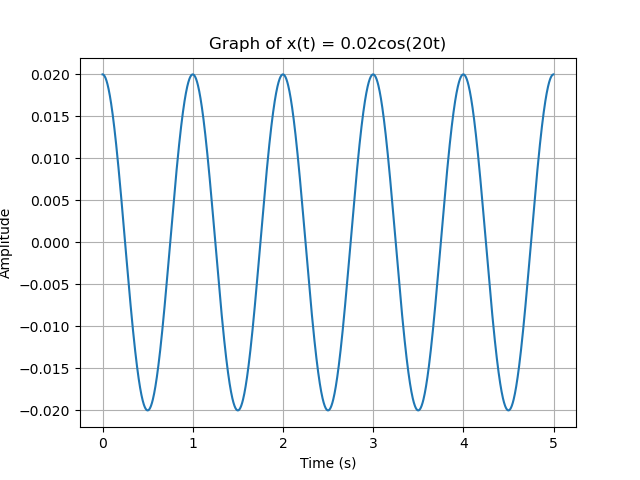
\includegraphics[width=1.1\linewidth]{ncert-physics/11/14/9/figs/analog1.png}
    \caption{plot of $x(t)$}
\end{figure}\\
(i) frequency of the oscillation
\begin{align}
    f&=\frac{\omega}{2\pi}\\\
    \implies f&=\frac{10}{\pi}
\end{align}
(iii)maximum speed of mass\\
\begin{align}
    x'(t)&=-A\omega\sin{\omega t}\\
  x'(t)\Bigr|_{max}&=A\omega\\
    \implies x'(t)\Bigr|_{max} &= 0.4 m/s
\end{align}
\begin{figure}[h!]
    \centering
    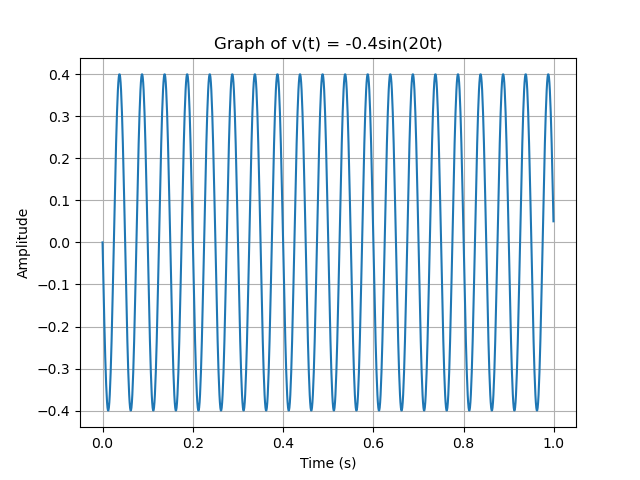
\includegraphics[width=1.1\linewidth]{ncert-physics/11/14/9/figs/analog2.png}
    \caption{plot of $x'(t)$}
\end{figure}\\
(ii)maximum accelaration of mass\\
\begin{align}
   x''(t)&=-A\omega^2 \cos{wt}\\
    x''(t)\Bigr|_{max}&=A\omega^2\\
    x''(t)\Bigr|_{max}&=8m/s^2
\end{align}
\begin{figure}[h!]
    \centering
    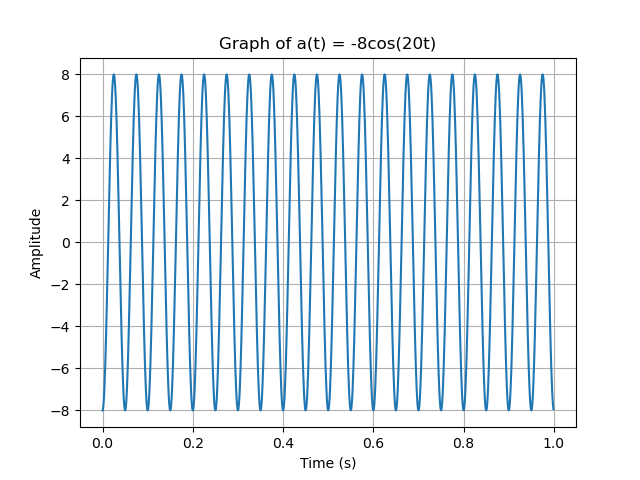
\includegraphics[width=1.1\linewidth]{ncert-physics/11/14/9/figs/analog3.png}
    \caption{plot of $x''(t)$}
\end{figure}
%\end{document}
